
% v2-acmsmall-sample.tex, dated March 6 2012
% This is a sample file for ACM small trim journals
%
% Compilation using 'acmsmall.cls' - version 1.3 (March 2012), Aptara Inc.
% (c) 2010 Association for Computing Machinery (ACM)
%
% Questions/Suggestions/Feedback should be addressed to => "acmtexsupport@aptaracorp.com".
% Users can also go through the FAQs available on the journal's submission webpage.
%
% Steps to compile: latex, bibtex, latex latex
%
% For tracking purposes => this is v1.3 - March 2012
\documentclass[prodmode,acmtecs]{acmsmall} % Aptara syntax
\usepackage[spanish,polish]{babel}
\usepackage[T1]{fontenc}
\usepackage{fancyvrb}
\usepackage{graphicx,hyperref}
\newcommand\cutout[1]{}


\usepackage[table]{xcolor}
\usepackage[utf8]{inputenc}
\usepackage[parfill]{parskip}
\usepackage{tabulary}
\PassOptionsToPackage{hyphens}{url}
\usepackage{hyperref}    
\usepackage[capitalize]{cleveref}


% Metadata Information
% !!! TODO: SET THESE VALUES !!!
\acmVolume{0}
\acmNumber{0}
\acmArticle{CFP}
\acmYear{0}
\acmMonth{0}

\newcounter{colstart}
\setcounter{page}{4}

\RecustomVerbatimCommand{\VerbatimInput}{VerbatimInput}%
{
%fontsize=\footnotesize,
fontfamily=\rmdefault
}


\newcommand{\UnderscoreCommands}{%\do\verbatiminput%
\do\citeNP \do\citeA \do\citeANP \do\citeN \do\shortcite%
\do\shortciteNP \do\shortciteA \do\shortciteANP \do\shortciteN%
\do\citeyear \do\citeyearNP%
}

\usepackage[strings]{underscore}



% Document starts
\begin{document}


\setcounter{colstart}{\thepage}

\acmArticle{CFP}
\title{{\huge\sc SIGLOG Monthly 252}

 July 2024}\author{ELLI ANASTASIADI\affil{Uppsala University, SE}\vspace*{-2.6cm}\begin{flushright}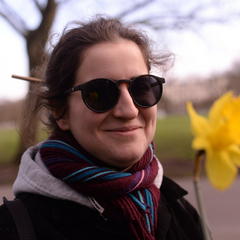
\includegraphics[width=30mm]{elli_anastasiadi.png}\end{flushright}}\begin{abstract}July 2024 edition of SIGLOG Monthly, featuring deadlines, calls and community announcements.
\end{abstract}


\maketitlee

\href{https://lics.siglog.org/newsletters/}{Past Issues}
 - 
\href{https://lics.siglog.org/newsletters/inst.html}{How to submit an announcement}
\section{Table of Contents}\begin{itemize}\item DEADLINES (\cref{deadlines}) 
 
\item SIGLOG MATTERS 
 
\begin{itemize}\item CHURCH AWARD 2024 (\cref{CHURCHAWARD2024})
\item CPP 2025 (\cref{CPP2025})
\end{itemize} 
\item CALLS 
 
\begin{itemize}\item ICLP/LPNMR-DC 2024 (CALL FOR PAPERS) (\cref{ICLPLPNMRDC2024})
\item ASPOCP 2024 (CALL FOR PAPERS) (\cref{ASPOCP2024})
\item LAMAS\&SR 2024 (CALL FOR PAPERS) (\cref{LAMASSR2024})
\item PhD Symposium iFM 2024 (CALL FOR PAPERS) (\cref{PhDSymposiumiFM2024})
\end{itemize} 
\item JOB ANNOUNCEMENTS 
 
\begin{itemize}\item University Assistant TU WIEN (\cref{UniversityAssistantTUWIEN})
\end{itemize} 
\item AWARDS 
 
\begin{itemize}\item CAV 2024 Award (\cref{CAV2024Award})
\end{itemize} 
\end{itemize}\section{Deadlines}\label{deadlines}\rowcolors{1}{white}{gray!25}\begin{tabulary}{\linewidth}{LL}ICLP/LPNMR-DC 2024:  & Aug 02, 2024 (Application) \\
ASPOCP 2024:  & Aug 08, 2024 (Abstract  deadline), Aug 15, 2024 (Paper  deadline) \\
University Assistant TU WIEN:  & Aug 08, 2024 (Application deadline) \\
LAMAS\&SR 2024:  & Aug 14, 2024 (Paper  deadline - EXTENDED) \\
PhD Symposium iFM 2024:  & Aug 23, 2024 (Paper  deadline) \\
CPP 2025:  & Sep 10, 2024 (Abstract Submission Deadline), Sep 17, 2024 (Paper Submission Deadline) \\
FSEN 2025:  & Oct 07, 2024 (Abstract Submission), Oct 14, 2024 (Paper Submission) \\
\end{tabulary}
\section{CHURCH AWARD 2024}\label{CHURCHAWARD2024}AWARD 

\begin{itemize}\item  The 2024 Alonzo Church Award for Outstanding Contributions to Logic and Computation is presented jointly to Thomas Ehrhard and Laurent Regnier for giving a logical and computational account of differentiation, bringing Taylor expansion to the Curry-Howard correspondence, which had a major impact on programming language semantics. 
 
\item  The awarded papers are:  
 
\begin{itemize}\item  Thomas Ehrhard. “Finiteness spaces”. In: Mathematical Structures in Computer Science 15.4 (2005), pp. 615–646. doi: 10.1017/S0960129504004645
\item  Thomas Ehrhard and Laurent Regnier. “The differential lambda-calculus”. In: Theoretical Computer Science 309.1-3 (2003), pp. 1–41. doi: 10.1016/S0304-3975(03)00392-X
\item  Thomas Ehrhard and Laurent Regnier. “Uniformity and the Taylor expansion of ordinary lambda-terms”. In: Theoretical Computer Science 403.2-3 (2008), pp. 347–372. doi: 10.1016/j.tcs.2008.06.001
\item  Thomas Ehrhard and Laurent Regnier. “B¨ohm Trees, Krivine’s Machine and the Taylor Expansion of Lambda-Terms”. In: Logical Approaches to Computational Barriers, Second Conference on Computability in Europe, CiE 2006, Swansea, UK, June 30-July 5, 2006, Proceedings. Ed. by Arnold Beckmann et al. Vol. 3988. Lecture Notes in Computer Science. Springer, 2006, pp. 186–197. doi: 10.1007/11780342\_20 
\item  Thomas Ehrhard and Laurent Regnier. “Differential interaction nets”. In: Theoretical Computer Science 364.2 (2006), pp. 166–195. doi: 10.1016/j.tcs.2006.08.003
\end{itemize} 
\item  The nominated papers introduced differential lambda-calculus and differential linear logic, together with the Taylor expansion of terms and proofs. The extension of the lambda-calculus with a derivation operator gives a syntactic account of differentiation, which reconciles the computational, logical, and algebraic notions of linearity. This allowed recasting Taylor expansion as a transformation of programs into superpositions of multilinear approximants, each capturing a finite computational behavior. The Taylor expansion has provided new and simpler proof methods to characterize the denotational and operational properties of programs. Differential linear logic similarly extends linear logic with new rules reflecting the logical structure of differentiation, yielding a sharper understanding of logical interaction. Differential linear logic has directly inspired unexpectedly effective accounts of differentiation in category theory, and strongly influenced current advances in higher-dimensional models of logic and computation. Differentiation has been instrumental in the design of new models of non-deterministic, probabilistic, quantum, or concurrent computation. After 20 years of intensive use, the concepts introduced in the awarded papers are time-tested and precious additions to the standard toolbox of the working linear logicians and programming language semanticists. 
 
\end{itemize}\section{CPP 2025: Certified Programs and Proofs}\label{CPP2025}  20-21 January 2025, co-located with POPL 2025, Denver, USA\\ 
  \href{https://popl25.sigplan.org/home/CPP-2025}{https://popl25.sigplan.org/home/CPP-2025}\\ 
CALL FOR PAPERS 

\begin{itemize}\item  Certified Programs and Proofs (CPP) is an international conference on practical and theoretical topics in all areas that consider formal verification and certification as an essential paradigm for their work. CPP spans areas of computer science, mathematics, logic, and education. 
 
\item  CPP 2025 (\href{https://popl25.sigplan.org/home/CPP-2025}{https://popl25.sigplan.org/home/CPP-2025}) will be held on 20-21 January 2025 and will be co-located with POPL 2025 in Denver, USA. CPP 2025 is sponsored by ACM SIGPLAN, in cooperation with ACM SIGLOG. CPP 2025 will welcome contributions from all members of the community. The CPP 2025 organizers will strive to enable both in-person and remote participation, in cooperation with the POPL 2025 organizers. 
 
\item  IMPORTANT DATES  
 
\rowcolors{1}{white}{gray!25}\begin{tabulary}{\linewidth}{LL}Abstract Submission Deadline:  & Sep 10, 2024 \\
Paper Submission Deadline:  & Sep 17, 2024 \\
Notification (tentative):  & Nov 19, 2024 \\
Camera Ready Deadline (tentative):  & Mid December 2024 (TBA) \\
Conference:  & Jan 20-21, 2025 \\
\end{tabulary}
 
  Deadlines expire at the end of the day, anywhere on earth. Abstract and submission deadlines are strict and there will be no extensions. 
 
\item  DISTINGUISHED PAPER AWARDS  
 
  Around 10% of the accepted papers at CPP 2025 will be designated as Distinguished Papers. This award highlights papers that the CPP program committee thinks should be read by a broad audience due to their relevance, originality, significance and clarity. 
 
\item  TOPICS OF INTEREST   
 
  We welcome submissions in research areas related to formal certification of programs and proofs. Please see \href{https://popl25.sigplan.org/home/CPP-2025#Call-for-Papers}{https://popl25.sigplan.org/home/CPP-2025\#Call-for-Papers} for a (non-exhaustive) list of topics.  
 
\item  SUBMISSION GUIDELINES 
 
  Prior to the paper submission deadline, the authors should upload their anonymized paper in PDF format through the HotCRP system at \href{https://cpp2025.hotcrp.com}{https://cpp2025.hotcrp.com} . The submissions must be written in English and provide sufficient detail to allow the program committee to assess the merits of the contribution. They must be formatted following the ACM SIGPLAN Proceedings format using the acmart style with the sigplan option, which provides a two-column style, using 10 point font for the main text, and a header for double blind review submission, i.e., \textbackslash{}documentclass[sigplan,10pt,anonymous,review]\{acmart\}\textbackslash{}settopmatter\{printfolios=true,printccs=false,printacmref=false\} . The submitted papers should not exceed 12 pages, including tables and figures, but excluding bibliography and clearly marked appendices. The papers should be self-contained without the appendices. Shorter papers are welcome and will be given equal consideration. We strongly encourage authors to read carefully our call for papers at \href{https://popl25.sigplan.org/home/CPP-2025#Call-for-Papers}{https://popl25.sigplan.org/home/CPP-2025\#Call-for-Papers} for instuctions on suplementary materials, the reviewing process, and copyrights. The official CPP 2025 proceedings will also be available via SIGPLAN OpenTOC (\href{http://www.sigplan.org/OpenTOC/#cpp}{http://www.sigplan.org/OpenTOC/\#cpp}). 
 
\item  CONTACT 
 
  For any questions please contact the two PC chairs: 
 
\begin{itemize}\item  Sandrine Blazy, University of Rennes (co-chair)
\item  Nicolas Tabareau, Inria (co-chair)
\end{itemize} 
\item  ORGANIZERS 
 
\begin{itemize}\item  Kathrin Stark, Heriot-Watt University (conference co-chair)
\item  Amin Timany, Aarhus University (conference co-chair)
\item  Sandrine Blazy, University of Rennes (PC co-chair)
\item  Nicolas Tabareau, Inria (PC co-chair)
\end{itemize} 
\end{itemize}\section{ICLP/LPNMR-DC 2024: Doctoral Consortium}\label{ICLPLPNMRDC2024}  October 13, 2024, Dallas, Texas, US\\ 
  co-located with International Conference on Logic Programming (ICLP 2024) and International Conference on Logic Programming and Non-monotonic Reasoning (LPNMR 2024)\\ 
  \href{https://sites.google.com/view/iclplpnmrdc2024}{https://sites.google.com/view/iclplpnmrdc2024}\\ 
CALL FOR PAPERS 

\begin{itemize}\item  The ICLP \& LPNMR Doctoral Consortium (DC) will take place during the 40th International Conference on Logic Programming (ICLP 2024) and the 17th International Conference on Logic Programming and Non-monotonic Reasoning (LPNMR 2024) in Dallas, Texas, US, on October 13, 2024. The DC will provide students and early career researchers with the opportunity to present and discuss their research directions, obtain feedback from both peers and experts in the field, and participate in mentoring sessions on how to prepare for a research career.  
 
  The DC is designed for students currently enrolled in a Ph.D. program, though we are also open to exceptions (e.g., students currently in a Master's program and interested in doctoral studies). Students at any stage in their doctoral studies are encouraged to apply for participation in the DC. Applicants are expected to conduct research in areas related to logic and constraint programming; topics of interest include (but are not limited to): 
 
\begin{itemize}\item  LP Foundations
\item  LP Languages
\item  Declarative Programming
\item  LP Implementation
\item  Related Paradigms and Synergies (e.g., Neuro-symbolic AI and Logic Programming)
\item  LP Applications.
\end{itemize} 
  The full call for papers can be found on the official website: \href{https://sites.google.com/view/iclplpnmrdc2024}{https://sites.google.com/view/iclplpnmrdc2024} 
 
\item  APPLICATION PROCESS 
 
  Submissions must be written in English and consist of: 
 
\begin{itemize}\item  a cover letter of the applicant, including a statement outlining the reasons for applying to the DC and how it will benefit the applicant;
\item  a research summary, prepared in EPTCS format (\href{http://info.eptcs.org/}{http://info.eptcs.org/}), that meets the following criteria. The body of the research summary (no more than 10 pages, excluding references, but 5 pages is fine as well!) should provide a clear overview of your research, its potential impact, and its current status. You are encouraged to include sections covering the following points: 1. Your complete name, address, and affiliation, 2. Introduction and problem description, 3. Background and overview of the existing literature,  4.Goals of the research, 5. Current status of the research, 6. Preliminary results accomplished (if any), 7. Open issues and expected achievements, 8. Bibliographical references, 
\end{itemize} 
  The application is to be submitted electronically in PDF format on the Easychair system, selecting the “Doctoral Consortium” track: \href{https://easychair.org/conferences/?conf=iclp2024}{https://easychair.org/conferences/?conf=iclp2024} 
 
\item  IMPORTANT DATES  
 
\rowcolors{1}{white}{gray!25}\begin{tabulary}{\linewidth}{LL}Application submission:  & Aug 02, 2024 \\
Notification to authors:  & Aug 26, 2024 \\
Camera-ready copy due:  & Sep 15, 2024 \\
DC event:  & Oct 13, 2024 \\
\end{tabulary}
 
\item  CONTACTS  
 
\begin{itemize}\item  Francesco Fabiano: ffabiano@nmsu.edu
\item  Martin Gebser: martin.gebser@aau.at
\end{itemize} 
\end{itemize}\section{ASPOCP 2024: 17th Workshop on Answer Set Programming and Other Computing Paradigms}\label{ASPOCP2024}  \href{https://sites.google.com/unical.it/aspocp2024/}{https://sites.google.com/unical.it/aspocp2024/}    \\ 
  October 12-13, Dallas, Texas\\ 
  Affiliated with ICLP 2024, 40th International Conference on Logic Programming\\ 
CALL FOR PAPERS 

\begin{itemize}\item  AIMS AND SCOPE 
 
  Since its introduction in the late 1980s, Answer Set Programming (ASP) has been widely applied to various knowledge-intensive tasks and combinatorial search problems. ASP was found to be closely related to SAT, which led to a new method of computing answer sets using SAT solvers and techniques adapted from SAT. This has been a much studied relationship, and is currently extended towards satisfiability modulo theories (SMT). The relationship of ASP to other computing paradigms, such as constraint satisfaction, quantified Boolean formulas (QBF), Constraint Logic Programming (CLP), first-order logic (FOL), and FO(ID) is also the subject of active research. Consequently, new methods of computing answer sets are being developed based on relationships to these formalisms. 
 
   Furthermore, the practical applications of ASP also foster work on multi-paradigm problem-solving, and in particular language and solver integration. The most prominent examples in this area currently are the integration of ASP with description logics (in the realm of the Semantic Web) and constraint satisfaction (which recently led to the Constraint Answer Set Programming (CASP) research direction). 
 
  A large body of general results regarding ASP is available and several efficient ASP solvers have been implemented. However, there are still significant challenges in applying ASP to real life applications, and more interest in relating ASP to other computing paradigms is emerging. This  workshop will provide opportunities for researchers to identify these challenges and to exchange ideas for overcoming them. 
 
\item  TOPICS 
 
  For a full list of topics see \href{https://sites.google.com/unical.it/aspocp2024/}{https://sites.google.com/unical.it/aspocp2024/} 
 
\item  SUBMISSIONS 
 
  The workshop invites two types of submissions: 
 
\begin{itemize}\item  original papers describing original research.
\item  non-original paper already published on formal proceedings or journals.
\end{itemize} 
  Original papers must not exceed 13 pages (excluding references) and must be formatted using the 1-column CEURART style available here. A ready-to-clone overleaf project containing a 1-column CEURART style is available here. Authors are requested to clearly specify whether their submission is original or not with a footnote on the first page. Authors are invited to submit their manuscripts in PDF via the EasyChair system at the link: \href{https://easychair.org/my/conference?conf=aspocp2024}{https://easychair.org/my/conference?conf=aspocp2024}. 
 
\item  IMPORTANT DATES 
 
\rowcolors{1}{white}{gray!25}\begin{tabulary}{\linewidth}{LL}Abstract submission deadline:  & Aug 08, 2024 \\
Paper submission deadline:  & Aug 15, 2024 \\
Notification:  & Sep 10, 2024 \\
\end{tabulary}
 
\item  PROCEEDINGS 
 
   Authors of all accepted original contributions can opt to publish their work in formal proceedings. Accepted non-original contributions will be given visibility on the conference web site including a link to the original publication, if already published. A selection of extended and revised versions of accepted papers could appear in a special issue. Extended versions of accepted non-original contributions, if not published in a journal yet, might be included in the issue. 
 
\item  WORKSHOP CO-CHAIRS 
 
\begin{itemize}\item  Francesco Pacenza, Department of Mathematics and Computer Science, University of Calabria, Italy
\item  Zeynep G. Saribatur, Institute of Logic and Computation, TU Wien, Austria  
\end{itemize} 
\end{itemize}\section{LAMAS\&SR 2024: International Workshop on Logical Aspects of Multi-Agent Systems and Strategic Reasoning}\label{LAMASSR2024}  November 2 - 4, 2024, Hanoi, Vietnam\\ 
  Co-located with KR 2024, International Conference on Principles of Knowledge Representation and Reasoning\\ 
  \href{https://conferences-website.github.io/lamassr24/}{https://conferences-website.github.io/lamassr24/}\\ 
CALL FOR PAPERS 

\begin{itemize}\item  OVERVIEW 
 
  Logic and strategic reasoning play a central role in multi-agent systems. Logic can be used, for instance, to express the agents' abilities, knowledge, and objectives. Strategic reasoning refers to algorithmic methods that allow for the development of good behavior for the agents of the system. At the intersection, we find logics that can express the existence of strategies or equilibria and can be used to reason about them. The LAMAS\&SR workshop merges two international workshops: LAMAS (Logical Aspects of Multi-Agent Systems), which focuses on all kinds of logical aspects of multi-agent systems from the perspectives of artificial intelligence, computer science, and game theory, and SR (Strategic Reasoning), devoted to all aspects of strategic reasoning in formal methods and artificial intelligence. Over the years the communities and research themes of both workshops got closer and closer, with a significant overlap in the participants and organizers of both events. For this reason, the two events have been unified under the same flag, formally joining the two communities. As such, the LAMAS\&SR workshop aims to bring together researchers working on different aspects of either logic or strategic reasoning in computer science, artificial intelligence, and multi-agent systems research, both from a theoretical and a practical viewpoint. 
 
\item  TOPICS OF INTEREST 
 
  For a full list of the relevant topics visit the LAMAS24 website.  
 
\item  IMPORTANT DATES 
 
\rowcolors{1}{white}{gray!25}\begin{tabulary}{\linewidth}{LL}Paper submission deadline - EXTENDED:  & Aug 14, 2024 \\
Acceptance notification:  & Aug 21, 2024 \\
Camera-ready version deadline:  & Sep 07, 2024 \\
LAMAS\&SR 2024 workshop:  & Nov 2nd, 3rd, or 4ths 2024 \\
\end{tabulary}
 
\item  SUBMISSION. 
 
  Authors are invited to submit extended abstracts of up to 4 pages plus 1 page for references only, in the format of the KR 2024 conference (KR24\_authors\_kit.zip). Both published and unpublished works are welcome. Submissions are subject to a single-blind review process (submissions should not be anonymous). Although there will be no formal proceedings, accepted extended abstracts will be available on the workshop website. Submissions must be in PDF and will be handled via CMT, using the following link: \href{https://cmt3.research.microsoft.com/LAMASSR2024}{https://cmt3.research.microsoft.com/LAMASSR2024} . Submissions from PC members are also allowed. Since the workshop will have informal proceedings, extended versions of the accepted papers can also be submitted elsewhere. 
 
\item  PROCEEDINGS  
 
  The informal proceedings will be available as a single PDF file from the workshop website. Extended and revised versions of the best papers presented at the workshop will be invited for a journal special issue. 
 
\item  COMMITTEES 
 
  Workshop Chairs:  
 
\begin{itemize}\item  Angelo Ferrando, University of Modena and Reggio Emilia
\item  Munyque Mittelmann, University of Naples Federico II
\item  Aniello Murano, University of Naples Federico II
\end{itemize} 
\end{itemize}\section{PhD Symposium iFM 2024: International Conference on integrated Formal Methods PhD Symposium}\label{PhDSymposiumiFM2024}  co-located with 19th iFM 2024\\ 
  12 November 2024, Manchester, United Kingdom\\ 
  \href{https://ifm2024.cs.manchester.ac.uk/phd-symposium.html}{https://ifm2024.cs.manchester.ac.uk/phd-symposium.html}\\ 
CALL FOR PAPERS 

\begin{itemize}\item  OBJECTIVE AND SCOPE 
 
  The iFM PhD symposium provides PhD students an opportunity to present and discuss their research in the fields of theory, implementation, integration or application of formal methods.  
 
\item  WHO CAN SUBMIT? 
 
  PhD students and young researchers at an early career stage (up to 2 years after PhD completion). 
 
\item  WHY TO SUBMIT AND PARTICIPATE? 
 
  Participants will have the possibility to present their research projects. Moreover: The doctoral symposium offers an excellent opportunity to introduce your work to fellow researchers in an international setting, and to get feedback from senior researchers in the field. The doctoral symposium lets you exchange knowledge and experiences with fellow PhD-students in a related topic -- both regarding research and regarding working towards an PhD.  
 
\item  WHAT TO SUBMIT? 
 
  There are several options for your submission: 
 
\begin{itemize}\item  Thesis Proposal Abstracts: summarize your research questions and outline your planned approach without needing to report experimental results. They are ideal for early-stage PhD students to get feedback on their research project during the initial planing and orientation phase. Abstracts have 2-3 pages, co-authors are allowed, and results may have been published previously if appropriately referenced. Indicate if also submitted to iFM2024.
\item  Result Reports: are short papers summarizing preliminary results of early-stage research.  Result Reports are short papers summarizing preliminary results of early-stage research. They should objectively report the addressed question, applied methods, and obtained results. Papers on unexpected results or ineffective methods are particularly welcome. Result Reports have 3-6 pages, co-authors are allowed, the work must be previously unpublished.
\item  Master summaries: are short papers summarizing the research question, method, and results of your impactful Master's thesis together with a discussion about possible next research steps. They are ideal for new and future PhD students to communicate their thesis results.  Master reports have 2-3 pages, an experienced supervisor should be a co-author, and results may have been published previously if appropriately referenced. Indicate if also submitted to iFM2024.
\end{itemize} 
  All submissions will be reviewed and accepted papers will be made publicly available in open-access online symposium proceedings. 
 
\item  SUBMISSION GUIDELINES 
 
  Multiple submissions by one author are not permitted. Submissions must be written in English and follow the CEUR-WS single-column formatting guidelines, available at: \href{http://ceur-ws.org/Vol-XXX/CEURART.zip}{http://ceur-ws.org/Vol-XXX/CEURART.zip}, or on overleaf \href{https://www.overleaf.com/latex/templates/template-for-submissions-to-ceur-workshop-proceedings-ceur-ws-dot-org/wqyfdgftmcfw}{https://www.overleaf.com/latex/templates/template-for-submissions-to-ceur-workshop-proceedings-ceur-ws-dot-org/wqyfdgftmcfw} 
 
  Please submit your contribution electronically in PDF via the EasyChair page: \href{https://easychair.org/conferences/?conf=ifm2024phd}{https://easychair.org/conferences/?conf=ifm2024phd} 
 
  All submissions will be peer reviewed, and will be evaluated based on their clarity and their potential to generate interesting discussions. Authors will get valuable feedback from more experienced reviewers. All types of contributions will benefit from feedback received during a dicussion at the workshop. Reviewing will be single blind, i.e, submissions need not be anonymized. 
 
\item  IMPORTANT DATES 
 
\rowcolors{1}{white}{gray!25}\begin{tabulary}{\linewidth}{LL}Paper submission deadline:  & Aug 23, 2024 \\
Acceptance notification:  & Sep 22, 2024 \\
Camera-ready version deadline:  & 7 Oct 2024 (AoE) \\
Symposium date:  & Nov 12, 2024 \\
\end{tabulary}
 
\item  PROGRAMME COMMITTEE 
 
\begin{itemize}\item  Erika Abraham, RWTH Aachen, Germany
\item  Ștefan Ciobâcă, UAIC Iași, Romania
\item  Mădălina Eraşcu, West University of Timisoara, Romania (co‑chair)
\item  Grigory Fedyukovich, Floria State University, USA
\item  Asmae Heydari Tabar, TU Darmstadt, Germany
\item  Eduard Kamburjan, University of Oslo, Norway
\item  Ondrej Lengal, Brno University of Technology, Czech Republic
\item  Philipp Rümmer, University of Regensburg, Germany
\item  Mattias Ulbrich, Karlsruhe Institute of Technology, Germany (co‑chair)
\end{itemize} 
  Further information available on the web page: \href{https://ifm2024.cs.manchester.ac.uk/phd-symposium.html}{https://ifm2024.cs.manchester.ac.uk/phd-symposium.html} 
 
\end{itemize}\section{University Assistant TU WIEN}\label{UniversityAssistantTUWIEN}JOB ANNOUNCEMENT 

\begin{itemize}\item  Institute of Logic and Computation, Research Unit Formal Methods in Systems Engineering 30 hours/week, limited to four years, estimated starting date is September 2024. The vacancy is advertised in German, as German skills are required due to teaching responsibilities. Details: \href{https://jobs.tuwien.ac.at/Job/236978}{https://jobs.tuwien.ac.at/Job/236978} 
 
Application deadline: Aug 08, 2024 
 
\end{itemize}\section{CAV 2024 Award}\label{CAV2024Award}AWARD 

\begin{itemize}\item  We are pleased to announce that the Computer Aided Verification (CAV) 2024 Award is given to: Clark Barrett, David Dill, Kyle Julian, Guy Katz, and Mykel Kochenderfer for their CAV 2017 paper titled “Reluplex: An Efficient SMT Solver for Verifying Deep Neural Networks”.  
 
  Deep neural networks are a state-of-the-art machine learning technology, which has become dominant in many areas within computer science. In a groundbreaking CAV 2017 paper, titled “Reluplex: An Efficient SMT Solver for Verifying Deep Neural Networks”, the authors, Clark Barrett, David Dill, Kyle Julian, Guy Katz, and Mykel Kochenderfer, developed a novel SMT-based algorithm, Reluplex, for verifying deep neural networks. The original algorithm was written to help verify the “Airborne Collision-Avoidance System for drone” system (ACAS-Xu).  Through Reluplex, the authors demonstrated, for the first time, that real-world neural networks could be verified. Reluplex could tackle neural networks that were over an order-of-magnitude larger as compared to previous verification techniques.  
 
  The Reluplex work had an immense impact on formal methods research, by creating a  highly active sub-field within the verification community, which is now center-stage in every major verification conference and is also subject to an annual competition dedicated specifically to the verification of neural networks (VNN-COMP). The Reluplex algorithm has been extended and enhanced, by the authors and by others, and the original paper has already accumulated more than 2000 citations (as of May 2024) – making it one of the most well-cited CAV papers in the past decades. Following their initial work, the authors continue to play a key role in solidifying the field of neural network verification. 
 
  For more information please check: \href{https://i-cav.org/2024/cav-award/}{https://i-cav.org/2024/cav-award/} 
 
  The CAV Award Committee: 
 
\begin{itemize}\item  Corina Pasareanu (Chair), NASA
\item  Rupak Majumdar, MPI-SWS
\item  Ranjit Jhala, University of California, San Diego
\item  Alessandro Cimatti, Fondazione Bruno Kessler
\end{itemize} 
\end{itemize}


\bigskip Links: \href{http://siglog.org/}{SIGLOG website}, \href{https://lics.siglog.org}{LICS website}, \href{https://lics.siglog.org/newsletters/}{SIGLOG Monthly}\end{document}